
%----------------------------------------------------------------------------
\chapter{Railway demonstrator system architecture}\label{chapter:RailwaySystem}
%----------------------------------------------------------------------------
In this chapter I want to describe the railway demonstrator system, which is shown in figure \ref{fig:overview}. This system's purpose is to simulate a real-life safety critical railway system, with basic functionalities and train collision detection. The demonstrator is based on a railway model stub which is extended with custom and off-the-shelf hardware, software components. 
\begin{figure}[h]
	\centering
	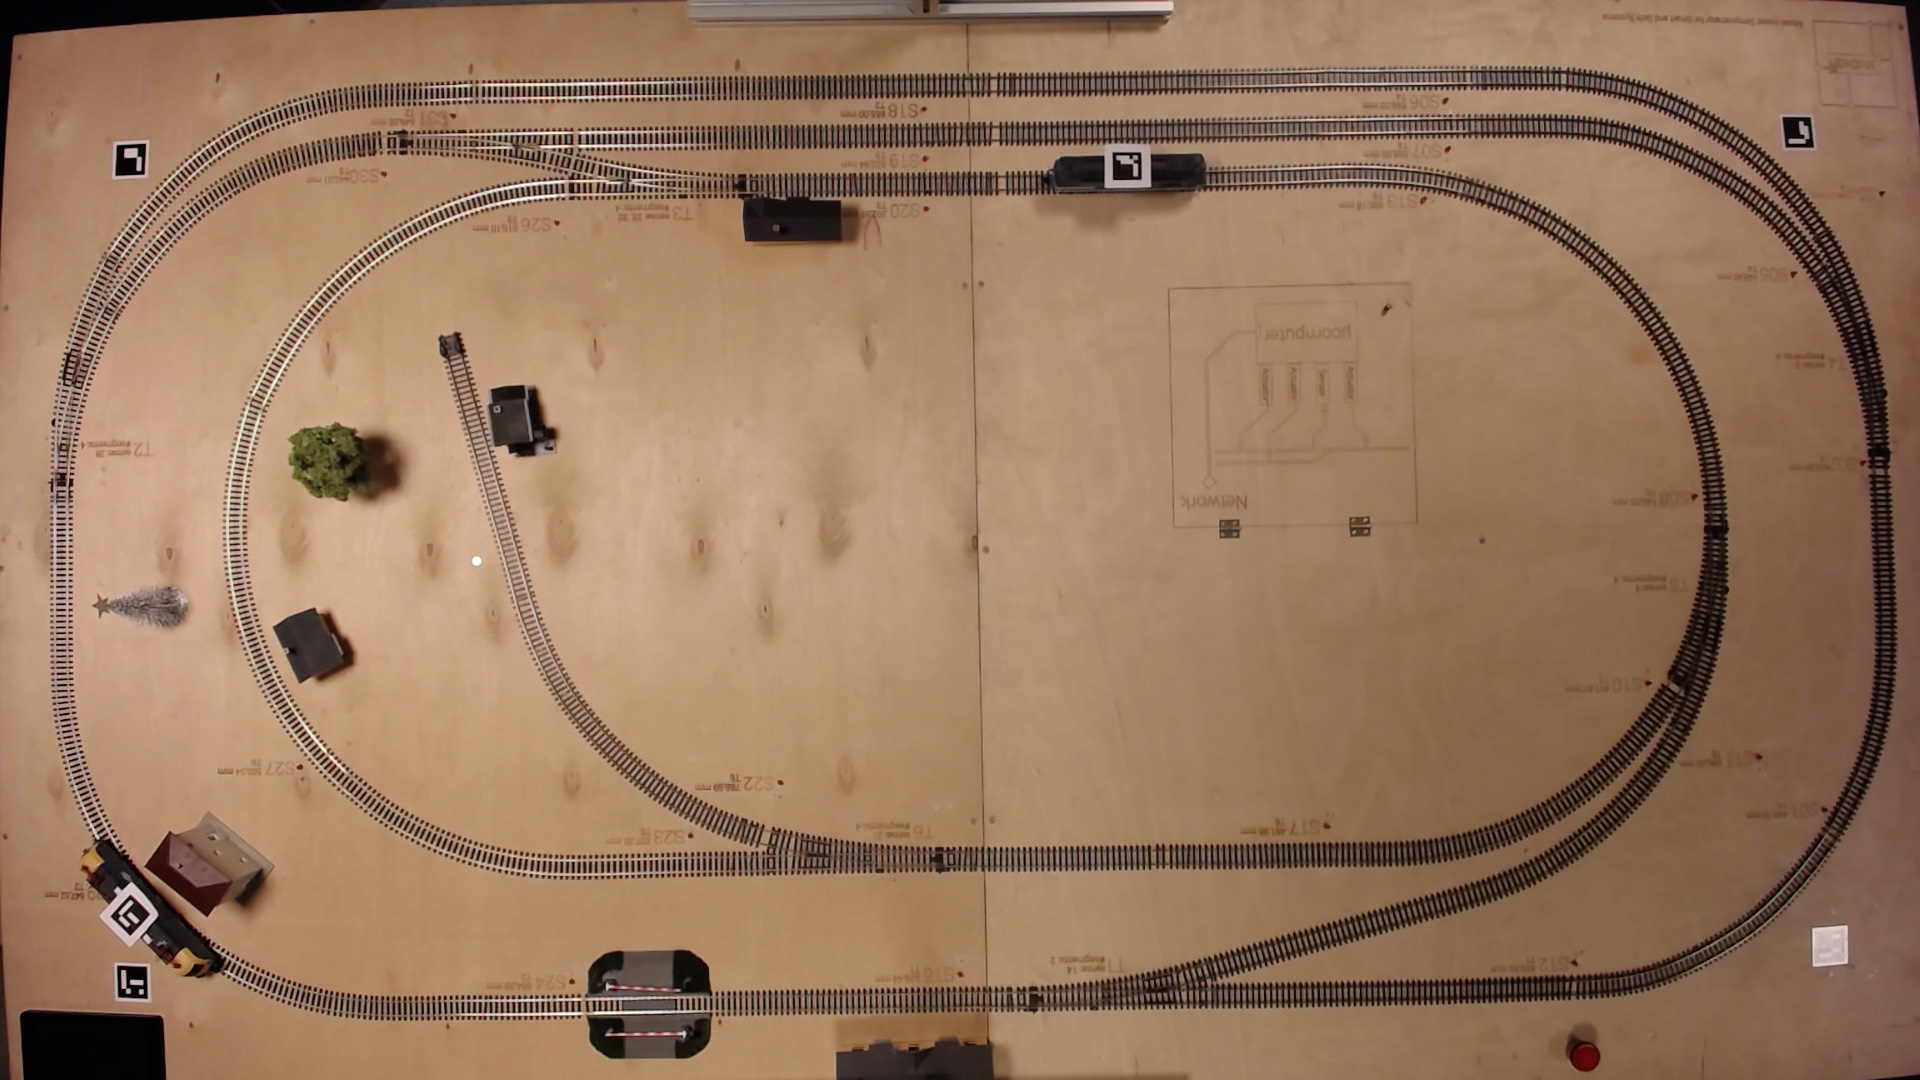
\includegraphics[width=150mm, keepaspectratio,  angle =180 ]{figures/modes3/overview.jpg}
	\caption{Railway system overview}
	\label{fig:overview}
\end{figure}

\section{Railway system basic components}
First of all I want to introduce the physical components and the basic process of the railway systems stub. There are 31 sections, with one blind track and 7 turnouts. The \ref{fig:layout} figure shows the layout of railway elements with the corresponding segment ids. Over all a segment means either section or turnout.
\todo[inline]{Create more visible figure about layout}

\begin{figure}[h]
	\centering
	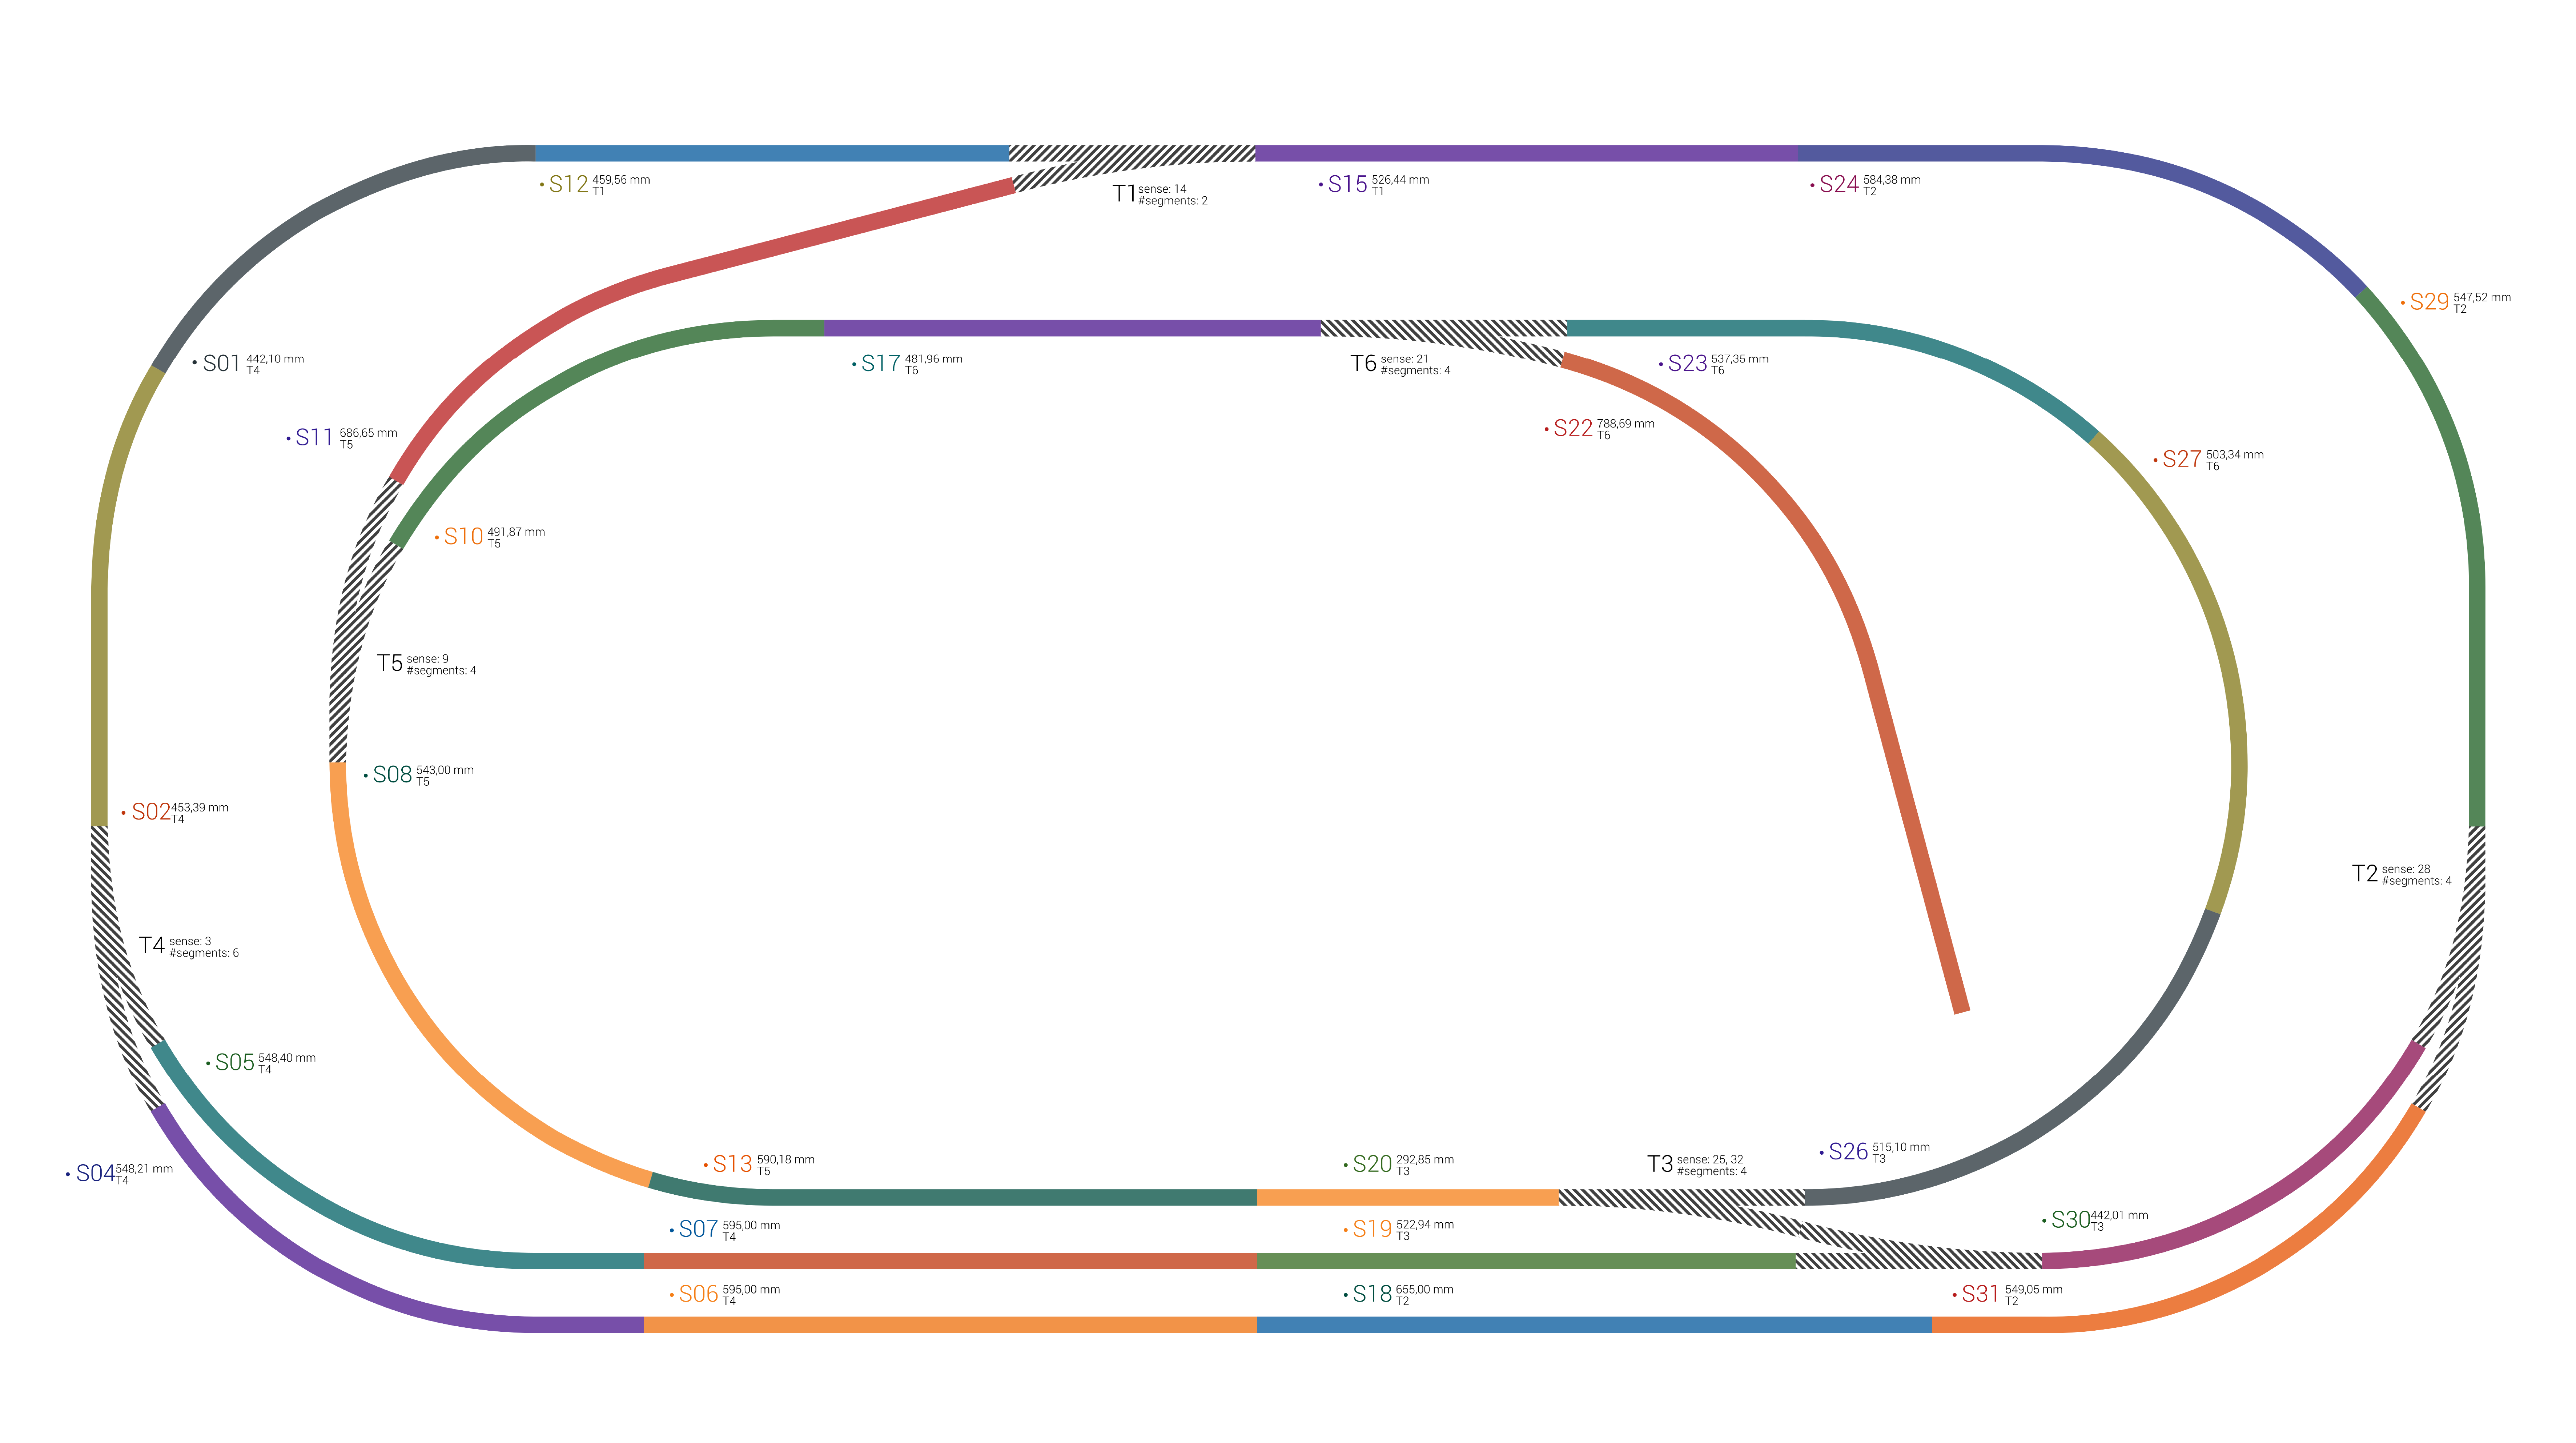
\includegraphics[width=150mm, keepaspectratio]{figures/modes3/layout2.png}
	\caption{Railway layout}
	\label{fig:layout}
\end{figure}

\paragraph{Section} 
First principal  element is a 15-20 cm long railroad. Each section is connected to 2 other sections, and wired to a command station which gives them sufficient power source for moving the trains. In the figure \ref{fig:layout} these sections are identified by \textit{SXX} strings, where \textit{XX} is two unique digits for this layout. Furthermore these numerals determines which bit shows this section's occupancy in the occupancy vector later (see section \ref{section:OccupancyDetection} for more information). On the \ref{fig:layout} figure for each section lengths and responsible BeagleBone Black ids are shown.

\paragraph{Turnout}
Second principal element is the turnout, which can differentiate 2 paths on the track as it can be seen on figure \ref{fig:turnoutDir}. The train which is going through a turnout can reach different sections depending on the state of the exact turnout. On the layout figure (\ref{fig:layout}) each of these elements are visible as gray dashed sections with the IDs. Each turnout ID starts with T and ends with a numeric (1..6). These IDs determines, which bit identifies the turnout's occupancy in the occupancy vector) and \textit{\#segments} as number of supervised sections by the BeagleBone Black (see section \ref{section:OccupancyDetection} for more information about occupancy vector).
\begin{figure}[!h]
	\centering
	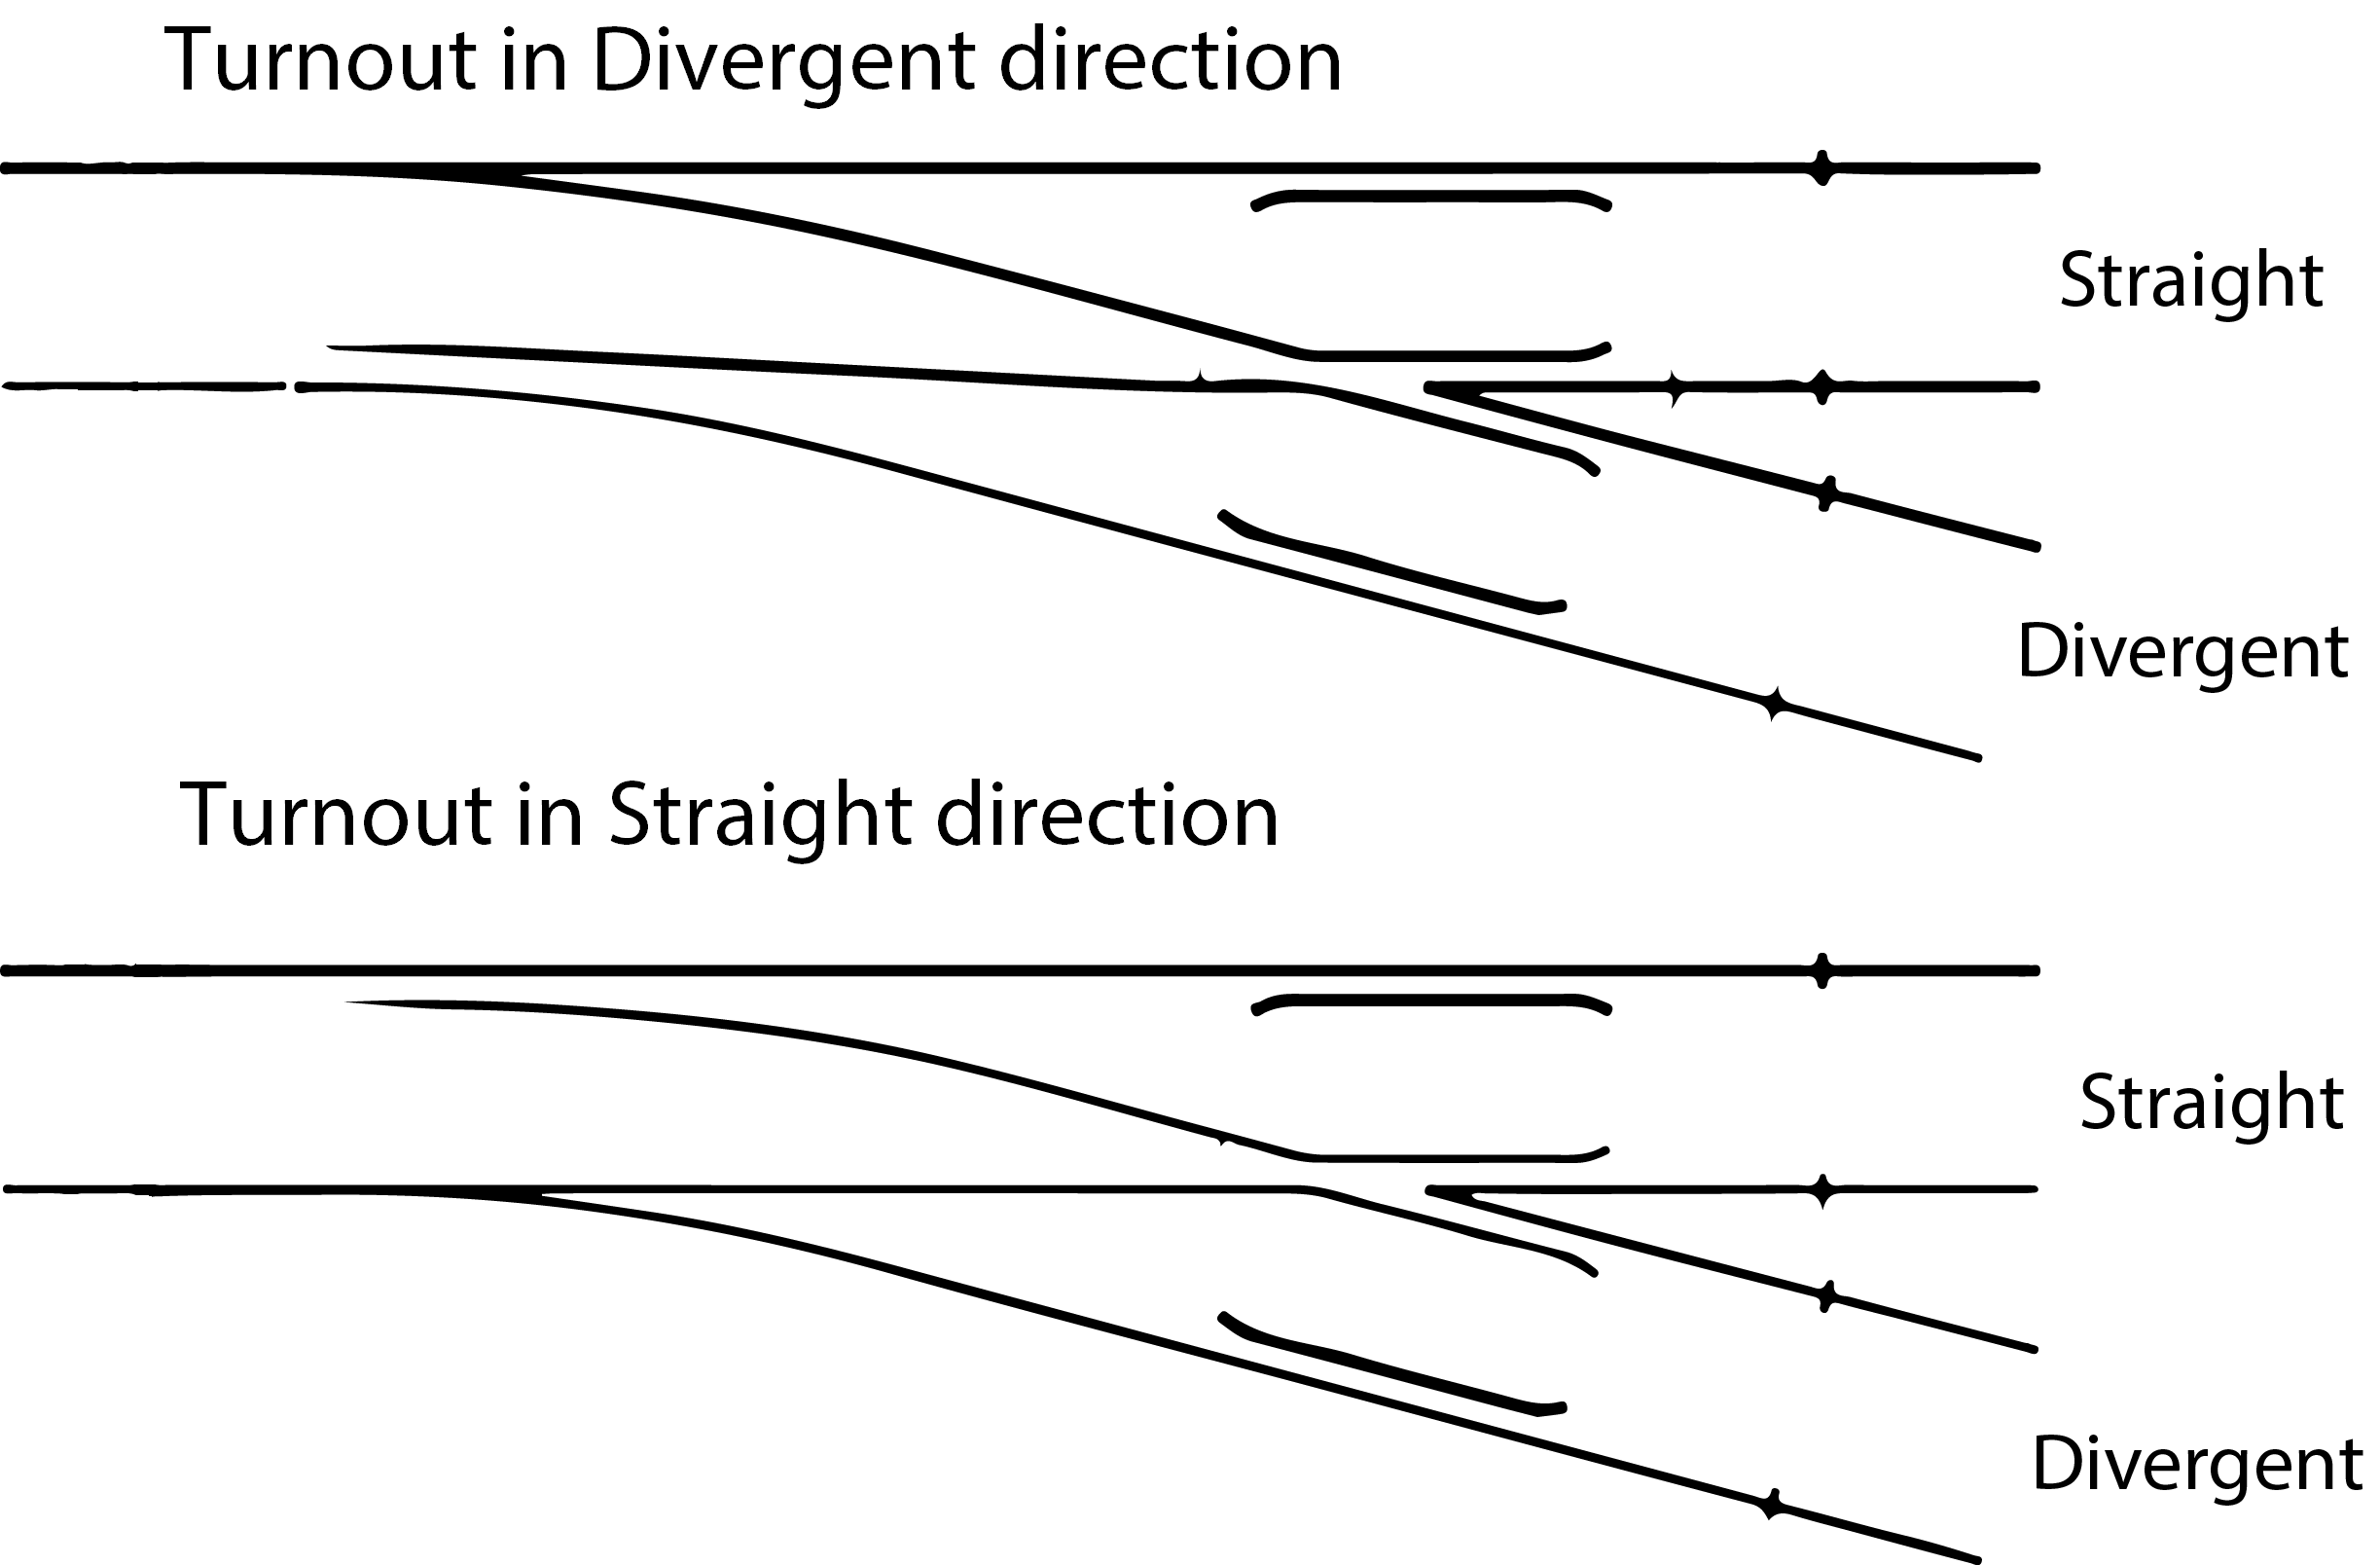
\includegraphics[width=150mm]{figures/modes3/turnout.png}
	\caption{Turnout directions}
	\label{fig:turnoutDir}
\end{figure}

\paragraph{Train} \label{par:trainScenarios}
There are 2 model trains in the system, which can move on the sections and turnouts. The first safety critical paradigm is to avoid a train collision on the track, for which the basic scenarios are the following. 

\todo[inline]{Move the collision scenarios to a new chapter}

First approach is that 2 trains are passing through the same turnout, from the same direction on different paths. It means that they are approaching the same section of the turnout, so they will collide like on the \ref{fig:LayoutT1-scenario1} figure.
\begin{figure}[!h]
	\centering
	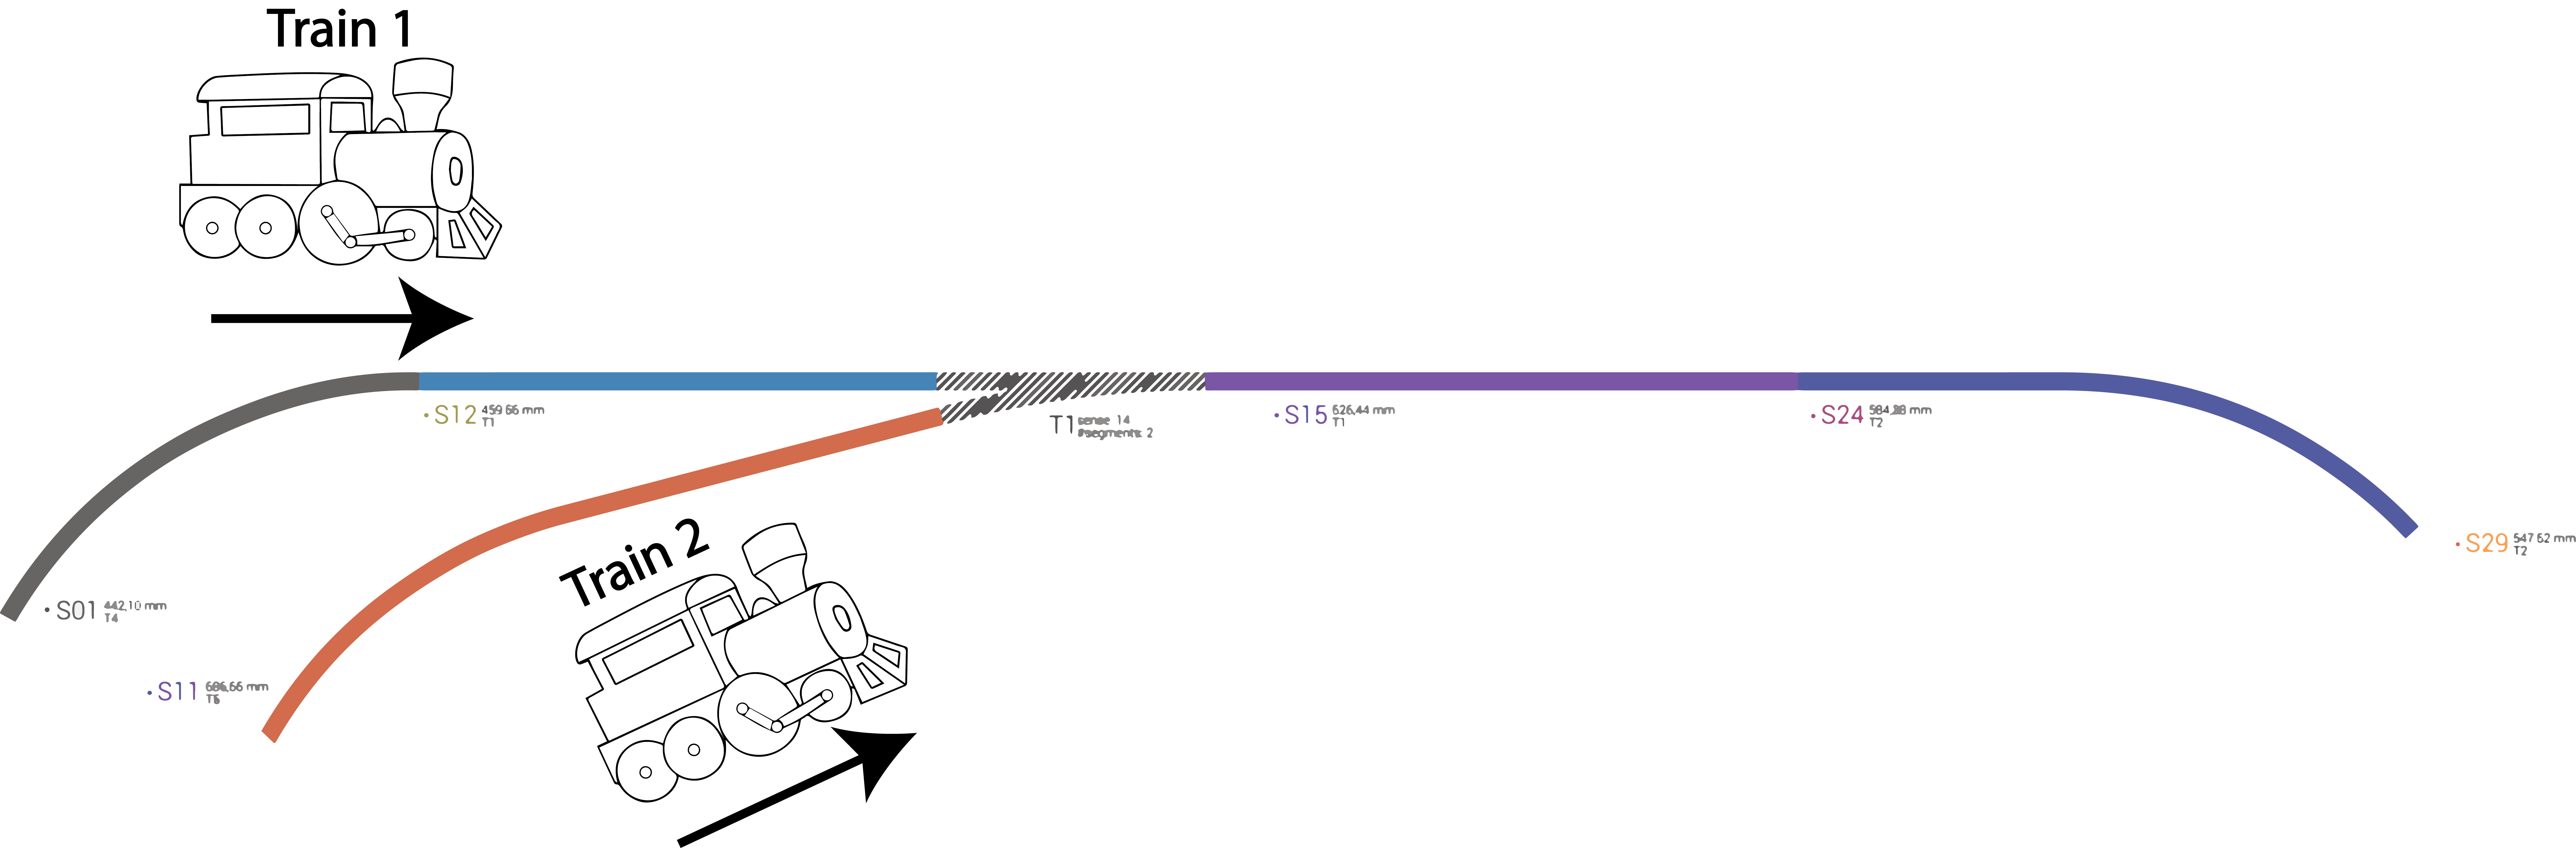
\includegraphics[width=150mm, keepaspectratio]{figures/modes3/layoutT1-scenario1.png}
	\caption{Turnout 1 collision scenario 1}
	\label{fig:LayoutT1-scenario1}
\end{figure}

Next possible scenario is shown in \ref{fig:LayoutT1-scenario2} figure, when \textit{Train 1} is going to the section where \textit{Train 2} is staying. Notice that no matter in which direction the \textit{Train 2} is moving or staying, it is a dangerous situation.
\begin{figure}[!h]
	\centering
	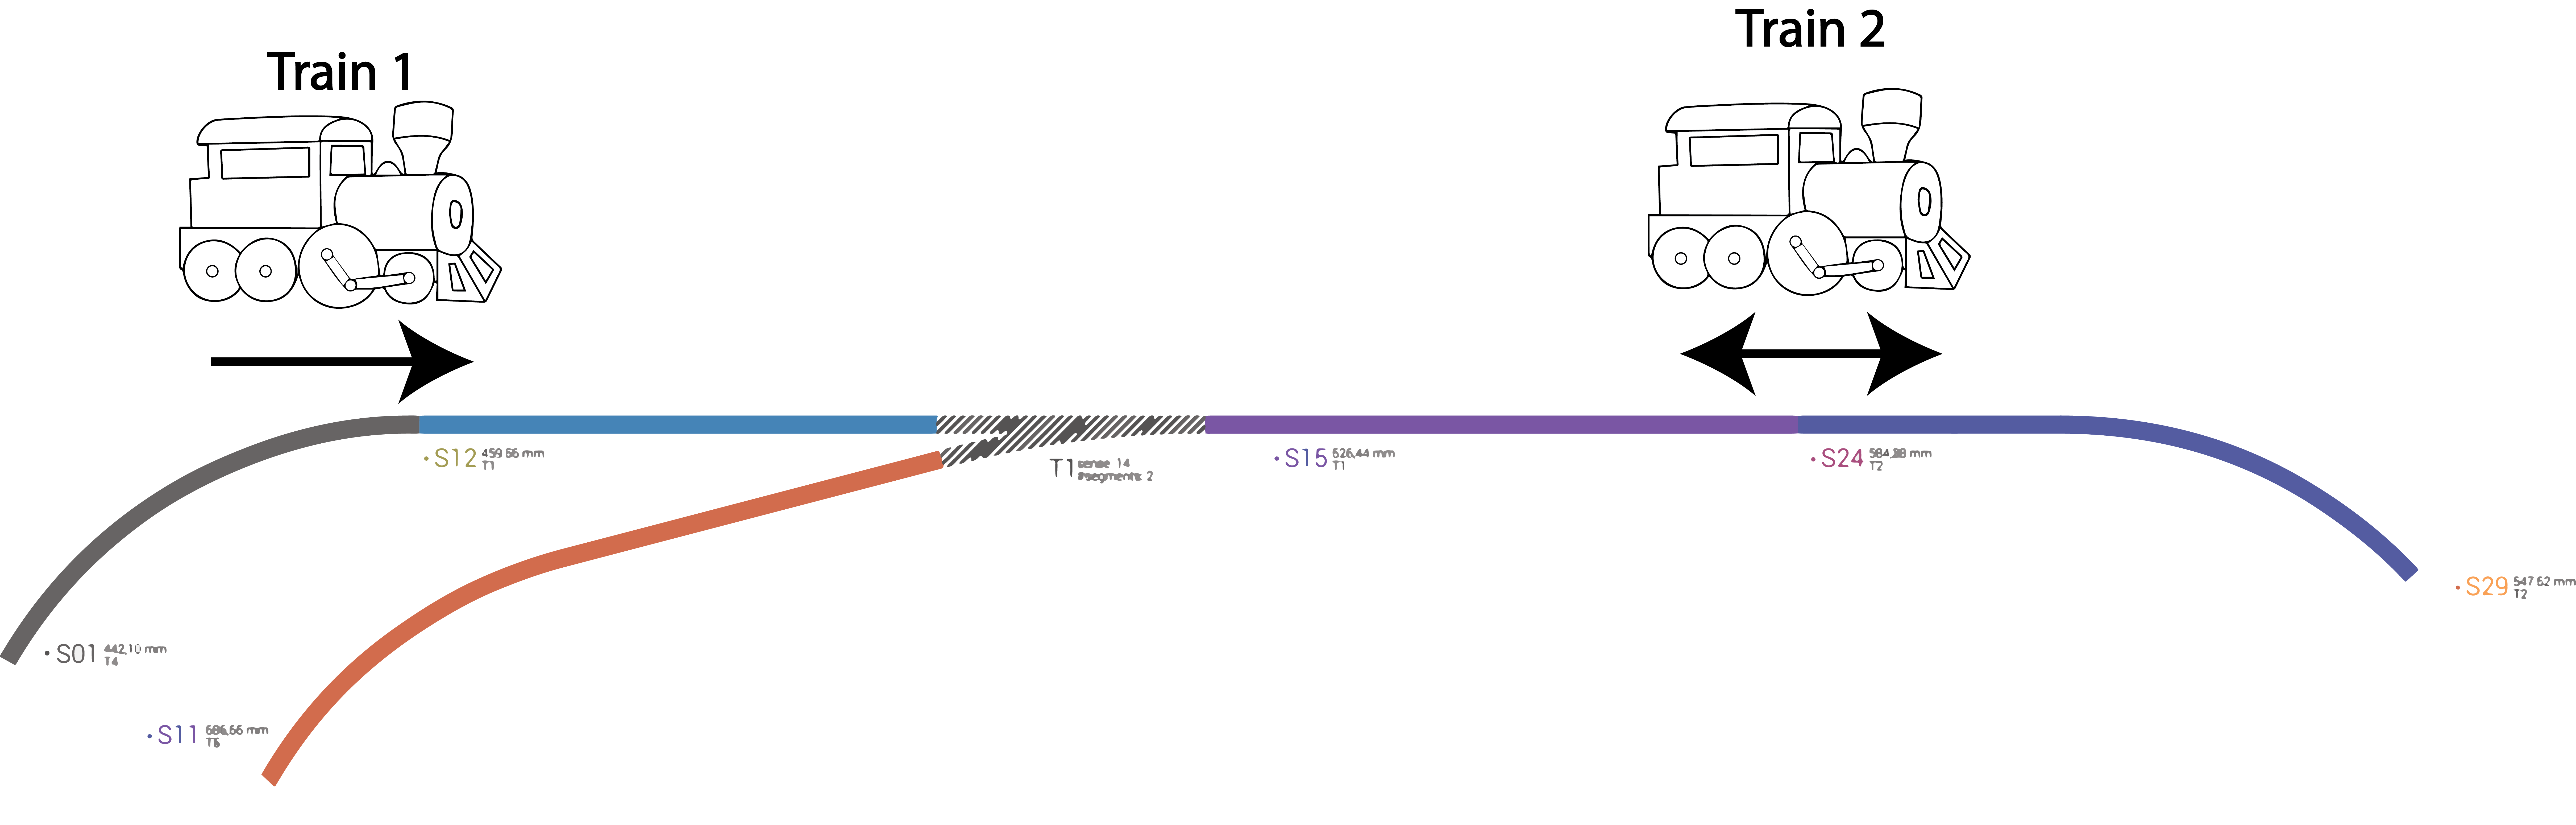
\includegraphics[width=150mm, keepaspectratio]{figures/modes3/layoutT1-scenario2.png}
	\caption{Turnout 1 collision scenario 2}
	\label{fig:LayoutT1-scenario2}
\end{figure}

\paragraph{Command Station} \label{basics:CS}
Supply power source for the sections which provides tension for the trains on the track.

\paragraph{Controller}
In connection with the \textit{Command Station} an XPressNet protocol \footnote{More details about XPressNet Protocol \url{http://www.lenzusa.com/1newsite1/Manuals/xpressnet.pdf}} based controller is attached to the system. This component's purpose is setting the direction and speed for each train on the track.

\section{Hardware extensions}
The basic hardware environment is not sufficient for controlling and analyzing purposes, therefore additional hardware elements have been designed to satisfy these requirements. In this section these platforms will be described in details. (The \ref{appendix:HWPictures} appendix contains pictures about the elements.)
\todo[inline]{Check if these infos are necessary and where to put them}
For modeling purposes I have used MagicDraw with Sysml plugin \cite{SysML}.

\subsection{Data processing units}
\begin{figure}[h]
	\centering
	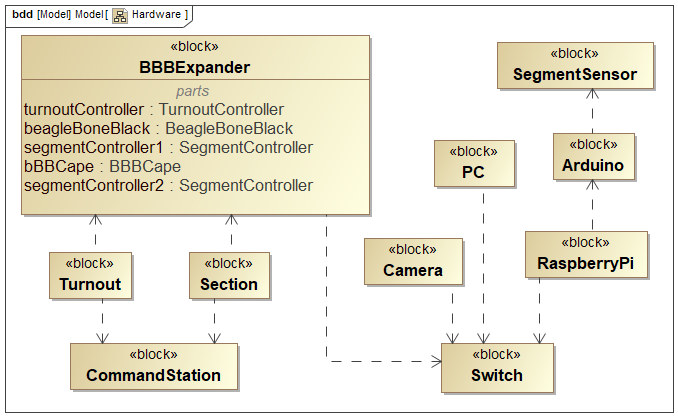
\includegraphics[width=150mm]{figures/modes3/Hardware.png}
	\caption{Hardware block definition diagram}
	\label{fig:Modes3HWBDD}
\end{figure}

\paragraph{BeagleBone Black (BBB)}
An industrial microcontroller platform which provides 4GB 8-bit eMMC on-board flash storage and 2x PRU 32-bit microcontrollers, which could satisfy the function for parallel monitoring. There are 6 BBB on the track connected to the railway, used for controlling and enabling/disabling each section.

\paragraph{Rapsberry Pi 3}
A Rapsberry Pi microcontroller is dedicated to handle most of the software components related to the Railway demonstrator system. It has twice as large computing capacity in RAM and also in CPU as BBB.

\paragraph{Arduino}
Dedicated hardware element for reading from the 6 DigiSens-8-S88 output data through S88 protocol (see \ref{par:SegmentSensor} section for details about this component). This communication layer requires proper timing conditions which the Arduino platform can satisfy.

\subsection{Custom hardware extensions}\label{section:CustomHW}
\paragraph{BeagleBone Black cape and expanders}\label{par:BBBcape}
The BeagleBone Black components expect 5VDC power source instead of 12VDC which our power station supplies. Because of that reason a so called cape have been created for each controller. Additionally the need for easy-to-use ports to attach additional circuits to the main board also have come up. The expanders could be used to extend the functionality of one BeagleBone unit, which is on the figure \ref{fig:capeSysml}. 
\todo[inline]{More suitable figure here for BBB expendable interfaces. For example: \url{https://github.com/FTSRG/BME-MODES3/wiki/HW-BeagleBone-expander-assignments}}

\begin{figure}[!h]
	\centering
	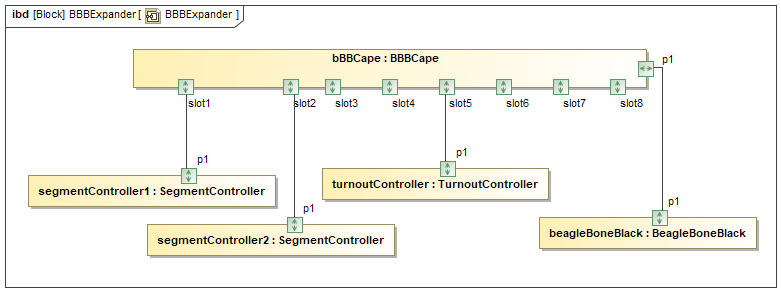
\includegraphics[width=150mm]{figures/modes3/BBBExpander.png}
	\caption{Layout and current attachment of cape and expander}
	\label{fig:capeSysml}
\end{figure}

Each cape have 8 general purpose expander slot, for which the pin layout is expressed in the following \ref{table:expander_pin_layout} table.

\begin{table}[!h]
	\caption{Pin layout}
	\label{table:expander_pin_layout}
	\begin{center}
		\renewcommand{\arraystretch}{1.5}
		\begin{tabu} to 0.5\textwidth { | X[c] | X[c] | X[c] | X[c] |}
			\hline
			pin3 & pin2 & pin1 & pin0 \\
			\hline
			3V3  & 5V  & Gnd  & 12V\\
			\hline
		\end{tabu}
	\end{center}
\end{table} 

\todo[inline]{Give proper details about G0-G15 pins, the table is not showing all of them like \url{https://github.com/FTSRG/BME-MODES3/wiki/HW-Expander-design}}  

The upper row of each connector is dedicated for GPIO connections. Two of the GPIO pins connected to the application processor and the remaining two GPIO pins are connected to the PRU unit.

With this setup, the PRU and the application processor can cooperate on hardware level.

\paragraph{Segment sensor}\label{par:SegmentSensor}
The DigiSens-8-S88 component is an off-the-shelf product, which can detect the occupancy for 8 segments. \footnote{More information about the product can be found here:\url{http://www.digitools.hu/termekek/erzekelok/digisens-8-s88}}.

\paragraph{Segment actuator}
Segment Actuator expanders are designed to stop a train on the corresponding segment. The concept behind this expander based on the Lenz Asymmetrical DCC and ABC functionality of train-decoders. \footnote{The following descriptions are based on \url{https://tonystrains.com/lenz-asymmetrical-dcc-and-abc/} article.}

%
%ABC (Automatic Brake Control) works in conjunction with Asymmetrical DCC. Asymmetrical DCC is a way to trigger ABC in the decoder. This gives the ability to stop trains at a section of the track with Asymmetrical DCC.

%\begin{figure}[!h]
%	\centering
%	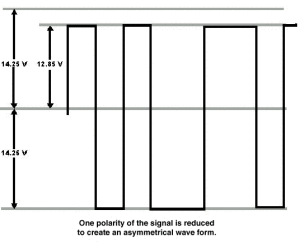
\includegraphics[width=100mm]{figures/modes3/DCC.png}
%	\caption{Asymmetric DCC voltages}
%	\label{fig:dcc}
%\end{figure}

%The Asymmetrical DCC signal is generated by offsetting one phase of the DCC signal. This signal then triggers the Automatic Brake Control in the decoder. This causes the engine to stop at the distance set up in the Constant Stopping Distance feature. We implemented this using five diodes. %connected in the form as shown in the figure below.
%\begin{figure}[h]
%	\centering
%	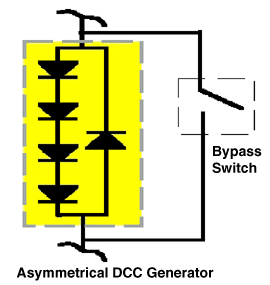
\includegraphics[width=50mm]{figures/modes3/abc.png}
%	\caption{Asymmetric DCC voltages}
%	\label{fig:abc}
%\end{figure}

The Segment Actuators uses this setup and also gives an interface (with GPIOs) to enable or disable this feature. Every Segment Actuator expander has two slots (A or B) and can enable or disable two segments. Each segment can be enabled setting two GPIOs to HIGH level, one connected to the PRU and one connected to the application processor.

\paragraph{Turnout actuator}
Turnout Actuator expanders can switch turnouts on the table between their states. Previously, we have managed to solve this with COTS (Commercial off-the-shelf) units, but in that case we were not able to query the position of the switch programmatically. This expander gives the ability for both switching the turnout and sensing its state.

The concept behind this unit is based on the fact, that turnout mechanism is working as a wire between the common (COM) pole and an other pole (STR or DIV) when switched in one position, therefore we can sense its state.

The electronic characteristics of the BeagleBone unit could not satisfy the switching process electrically, thus we had to use a micro-controller (an Atmega328 MCU). Also, the state-sensing process is based on Analog to Digital Converters, which are also integrated into the MCU.

\textbf{Usage}
The MCU has 2 inputs and 2 outputs connected to the expander connector as shown in the table below.
\begin{center}
	\renewcommand{\arraystretch}{1.5}
	\begin{tabu} to 1.0\textwidth {X[c] X[c] X[c] X[c]}
		\toprule
		Pin 0                                  & Pin 1                                   & Pin 2                           & Pin 3                             \\ \midrule
		Turnout switching to Straight position & Turnout switching to Divergent position & Turnout state sensing (Straing) & Turnout state sensing (Divergent) \\
		INPUT for the MCU                      & INPUT for hte MCU                       & OUTPUT for the MCU              & OUTPUT for the MCU                \\ \bottomrule
	\end{tabu}
\end{center}


\section{Software components}\label{section:CustomSW}
\todo[inline]{update the figure with traindetector and delete physical controllers}
\begin{figure}[h]
	\centering
	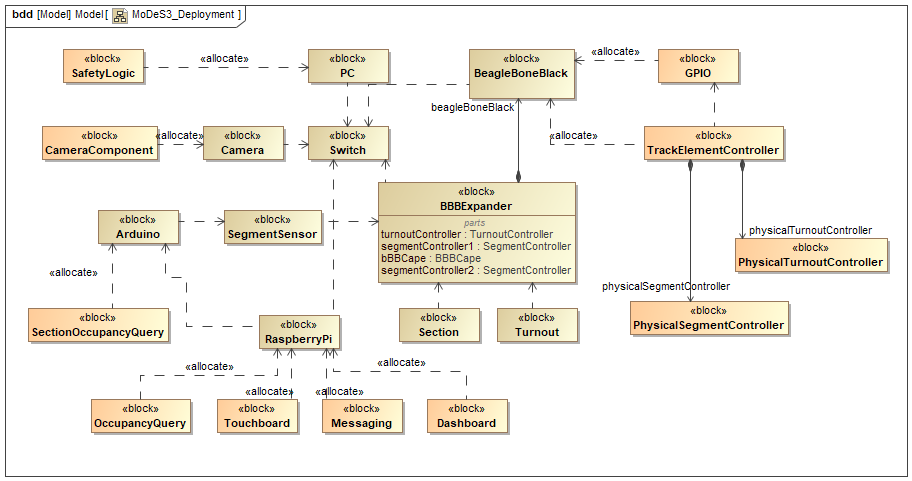
\includegraphics[width=150mm]{figures/modes3/MoDeS3_Deployment1.png}
	\caption{Software components deployment to hardware elements}
	\label{fig:Modes3Deployment}
\end{figure}

\subsection{Occupancy detection elements} \label{section:OccupancyDetection}
\paragraph{Section Occupancy Query}
Responsible for debouncing the 32bit long occupancy vector with proper timing conditions regarding S88 protocol and forward this 32bit to \textit{Occupancy Query} through usb connection. Computed data contains the occupancy information for each track element (section or turnout) per one bit.
\paragraph{Occupancy Query}
In connection with the \textit{Section Occupancy Query} process the occupancy state for the whole track. Only if the state has changed, it sends occupancy change message to the MQTT topic with the track element id and new occupancy state.

\subsection{Track segment control elements}
\paragraph{GPIO}
Handles the GPIO pin changes and commands for each extension point of the BBB cape (see \ref{par:BBBcape} section for details about BBB cape and expanders).
\paragraph{Track Element Controller}
On each BeagleBone Black microcontroller there is a controller, which executes the turnout and segment operations for the supervised sections. To satisfy this functionality this controller forwards commands to the corresponding Physical Segment or Turnout Controllers, which communicates with GPIO managers. Consequently with this platform specific software, we are able to enable or disable sections and set turnout directions.
\paragraph{Train Detector}
Train detector and locomotive length measurer using infrared sensors.

\subsection{Track control and supervisor elements}
\paragraph{XPressNet}
Protocol for sending messages to the \textit{Command Station} component, therefore we can extend the communication form for controlling the track. In the current layout there is a controller and web-based opportunity for controlling.
\paragraph{Dashboard}
Model railway track dashboard implementation, where we can manipulate the track elements. In Addition this component is instantiated only once, and up for the whole time while the track is in use. Consequently we can reach one common dashboard from the web and it contains the actual occupancy and track element status.
\paragraph{Touch board}
Dashboard for the model railway track, with focus on touchable elements, that can be controlled.
\paragraph{Safety Logic}
In the MODES$^3$ safety critical project we want to avoid the collision of model trains, therefore the safety logic software component detects these critical scenarios by Viatra Query \cite{Viatra} patterns and act the necessary action (for example disable a section).

\subsection{Communication}
Each software component share information about the railroad system through the messaging software element, which is based on protobuf messages and provides high-level designed API with MQTT for this purpose. 
\begin{figure}[!h]
	\centering
	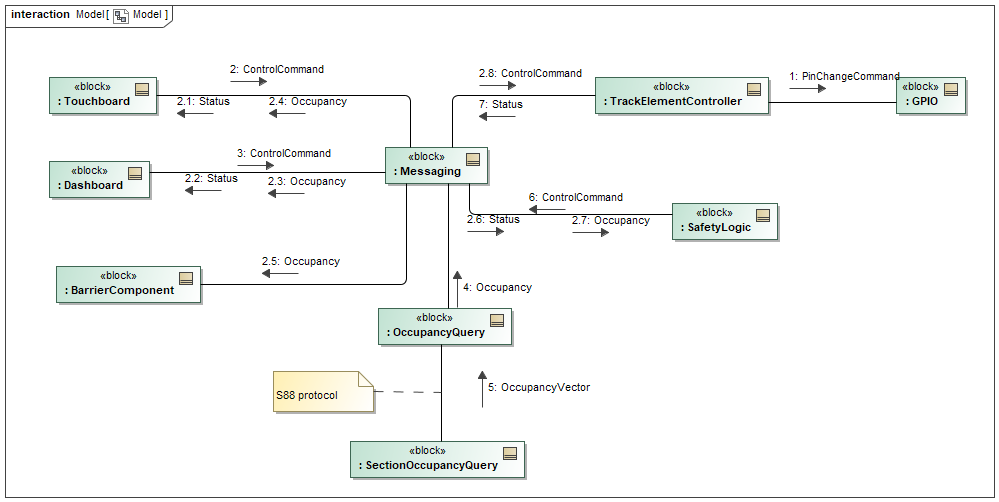
\includegraphics[width=150mm, keepaspectratio]{figures/modes3/CommunicationModel.png}
	\caption{Communication between software components}
	\label{fig:communicationModel}
\end{figure}

Separated topics are created for different information flow, and any component can subscribe for these topics. Basically on all topic, the information reporting is change based, so all components sending an information message to the dedicated topic when their state have changed (like occupancy changed or turnout changed). In opposite to that, there is a \textit{SendAllStatusCommand} which is a request for every component to send their actual status.

I will now list the specific MQTT topics and the connected software components to that, so basically what kind of information is flowing on them. (See software component connections on figure \ref{fig:communicationModel})

\paragraph{Segment Occupancy topic}
On this topic the \textit{Occupancy Query} component sending information whether an occupancy state is changed on any segment. (Notice that a segment can also be a section or a turnout too.) Most of the components are subscribed for this information topic so the \textit{Touch board}, \textit{DashBoard}, \textit{Barrier} (only for the supervised segments), \textit{Track Element Controller} and \textit{Safety Logic}.

\paragraph{Segment and Turnout Command topic}\label{par:MQTTTopicCommand}
Basically the \textit{Track Element Controller} process and accomplish these commands, and \textit{Touch board}, \textit{Dashboard} and \textit{Safety Logic} components can give these instructions.

\paragraph{Segment and Turnout Status topic}\label{par:MQTTTopicStatus}
For every command the \textit{Track Element Controller} will give a status acknowledgment message with the new state of the turnout or section. In this way the \textit{Touch board}, \textit{Dashboard} and \textit{Safety Logic} elements will be informed about the latest and current state.

\paragraph{CV topic}
The camera notification is communicated on that topic, which is received by the \textit{Safety Logic}.

\paragraph{ALL topic}
For this specific topic all the components in the system are subscribed, and information about train controlling and \textit{Command Station} related messages are shared.

\subsection{Complementary elements}
\paragraph{Barrier} 
Sends open/close commands to the barrier over the network, depending on the occupancy of supervised segments.
\paragraph{Leapmotion}
Software component for converting gestures into special movements for changing the speed of a specific train.

\section{Safety-critical functionalities}\label{section:SC-Functionalities}

\todo[inline]{Maybe figure of the Sw-Hw sysml for each paragraph}

\paragraph{Occupancy detection}\label{par:FunctionOccupancyDetection}
In order to know where are the trains on the track, we first must know which track elements (section or turnout) is occupied. This attribute can be determined whether the specific section has power consumption, which is used by a train on it. The actual detection is made by the \textit{DigiSens-8-S88} sensing element. The demonstration railway system have four sensing elements, and they are connected to an \textit{Arduino}'s S88 port. This microcontroller computes basic calculations by \textit{Section Occupancy Query} C++ software component and forwards the 32-bit occupancy vector information (actual state of every track element) to the \textit{Occupancy Query} via USB connection. The \textit{ Occupancy Query} Java component on the \textit{Rapsberry Pi} stores the previous occupancy state, and sends a status information to the \textit{Segment Occupancy} topic about every change.

\paragraph{Track element controlling}\label{par:FunctionTEC}
For safety critical purposes in any collision scenario it is a good manner to disable all track elements, which is affected in the critical scenario. To make this switch possible, we have to cut the electric circle between the segment and \textit{Command Station}. The \textit{Section Controller} hardware element have been developed for changing a section,  the \textit{Turnout Controller} is responsible for changing a turnout. These hardware elements are attached to a \textit{BBB cape}, which is designed for supplying extension ports for BBB. In software point of view, through GPIO pins (specific file writing), we can give impulses from the BBB to the section or turnout. Therefore a \textit{GPIO manager} component is responsible for that in connection with the \textit{Track Element Controller component}. Both of them are Java components and deployed to the BBB microcontrollers.

\paragraph{Safety critical verification}
Because of the network communication, it is easy to connect a \textit{safety logic} in the system. In addition a camera component is reading the position of the trains on the track. If the \textit{Safety Logic} detects an unsafe scenario from the occupancy detection or camera, it switches off the affected elements by a \textit{Track Element Controller} signal.

\section{Requirements}\label{section:REQ}
In this section I want to collect the specific requirements for the above described elements in the system, not considering market products. I have categorized them into functional and component groups.

\todo[inline]{Create sysml diagrams for better overview}

\paragraph{Hardware extensions}
\begin{enumerate}[label=REQ-BBB-\arabic*, leftmargin=*, format=\small]
	\item The BeagleBone Black cape must supply 5VDC power source.
	\item The BeagleBone Black expander must provide further options to attach additional hardware elements. The purpose is to access application processor and PRU unit pins of BeagleBone Black with more elements.
\end{enumerate}

\begin{enumerate}[label=REQ-SA-\arabic*, leftmargin=*, format=\small]
	\item The Segment actuator must stop the train on the given section with the built in \textit{Command Station} (see section \ref{basics:CS}).
\end{enumerate}

\begin{enumerate}[label=REQ-TA-\arabic*, leftmargin=*, format=\small]
	\item The Turnout actuator must switch the corresponding turnout between divergent and straight states.
	\item The Turnout actuator must sense the given actual state of the turnout.
\end{enumerate}

\paragraph{Occupancy detection software elements}
\begin{enumerate}[label=REQ-SOQ-\arabic*, leftmargin=*, format=\small]
	\item The Section Occupancy Query must collect the occupancy information together from all segments on the track. \label{req:SOQ}
\end{enumerate}

\begin{enumerate}[label=REQ-OCQ-\arabic*, leftmargin=*, format=\small] 
	\item The Occupancy Query software element must determine whether a train is on the specific segment (results a free occupancy state) or not (results an occupied occupancy state) for each segment,  \label{req:OCQ-1}
	\item The Occupancy Query software element must send a message when an occupancy state changed for any segment. The component must send all the present section's occupancy states. \label{req:OCQ-2}
\end{enumerate}

\paragraph{Track segment controller software elements}
\begin{enumerate}[label=REQ-GPIO-\arabic*, leftmargin=*, format=\small] 
	\item The GPIO software element must change the GPIO pins between their input and output states. \label{req:GPIO}
\end{enumerate}

\begin{enumerate}[label=REQ-TEC-\arabic*, leftmargin=*, format=\small]
	\item The Track Element Controller must be able to enable and disable each section with a specific command. \label{req:TEC-1}
	\item The Track Element Controller must be able to change each turnout's direction to straight or divergent state. \label{req:TEC-2}
\end{enumerate}

\todo[inline]{Looks like it can be deleted, because it is not in production, was just an experiment}
\begin{enumerate}[label=REQ-TD-\arabic*, leftmargin=*, format=\small]
	\item The Train Detector must identify the length and speed of a specific train. \label{req:TD}
\end{enumerate}

\paragraph{Track control and supervisor software elements}

\begin{enumerate}[label=REQ-DB-\arabic*, leftmargin=*, format=\small]
	\item The Dashboard must observe the track element states throughout the whole life-cycle. \label{req:DB-1}
	\item The Dashboard must be able to change all turnout states. \label{req:DB-2}
	\item The Dashboard must be able to change each turnout state separately. \label{req:DB-3}
	\item The Dashboard must be able to enable and disable all segments on the track. \label{req:DB-4}
	\item The Dashboard must be able to enable and disable each segment on the track, separately. \label{req:DB-5}
\end{enumerate}

\todo[inline]{DB req can be compressed together?}

\begin{enumerate}[label=REQ-SL-\arabic*, leftmargin=*, format=\small]
	\item The Safety Logic software must avoid safety-critical scenarios on the track. \label{req:SL-1}
	\todo[inline]{Explain safety-critical scenarios here or just make a link?}
	\item The Safety Logic must ensure that a train must not go on a disabled segment. \label{req:SL-2}
	\item The Safety Logic must ensure that a train must stop in the straight direction of the turnout, when the turnout is in divergent state. \label{req:SL-3}
	\item The Safety Logic must ensure that a train must stop in the divergent direction of the turnout, when the turnout is in straight state. \label{req:SL-4}
\end{enumerate}
	


%\section{TBD : Component level test plans}
%\todo[inline]{Link the test conditions to requirements!}
%
%\paragraph{Custom hardware elements}
%
%\begin{enumerate}[label=TEST-BBB-\arabic*, leftmargin=*, format=\small]
%	\item Measure BeagleBone Black cape power output voltage that it is matching with the required 5VDC.
%	\item \todo[inline]{How to test expander processor attachment?}
%\end{enumerate}
%
%\begin{enumerate}[label=TEST-SA-\arabic*, leftmargin=*, format=\small]
%	\item Check that when the segment actuator got stop signal, the train stopped on the corresponding section.
%\end{enumerate}
%
%\begin{enumerate}[label=TEST-TA-\arabic*, leftmargin=*, format=\small]
%	\item Change one Turnout's state from divergent to straight and verify that the new state is in straight.
%	\item Change one Turnout's state from straight to divergent and check that the new state is in divergent.
%\end{enumerate}
%
%\begin{enumerate}[label=TEST-TD-\arabic*, leftmargin=*, format=\small]
%	\item Retrieve the actual state for one Turnout and check its correctness.
%\end{enumerate}
%
%\paragraph{Occupancy detection software elements}
%\begin{enumerate}[label=Test-SOQ-\arabic*, leftmargin=*, format=\small]
%	\item Collect the occupancy informations on the track with the Section Occupancy Query software in the following scenarios:
%	\begin{enumerate}
%		\item 1 train is on the turnout T3
%		\item 1 train is on the turnout T1
%		\item 1 train is on the segment S02
%		\item 1 train is on the segment S15
%		\item 1 train is on the segment S18
%		\item 1 train is on the segment S22
%	\end{enumerate}
%
%	\item Verify that the occupancy information is contains all segment occupancy informations.
%\end{enumerate}
%\begin{enumerate}[label=TEST-OCQ-\arabic*, leftmargin=*, format=\small]
%	\item Change one or more segment's state and verify that a new occupancy information is sent with all current segment's states.
%\end{enumerate}
%
%\paragraph{Track segment controller elements}
%\begin{enumerate}[label=Test-GPIO-\arabic*, leftmargin=*, format=\small]
%	\item Change the GPIO pin to output and verify that the pin can be used for outgoing communication from the segment.
%	\item Change the GPIO pin to input and verify that the pin can be used for incoming communication from the segment.
%\end{enumerate}
%
%\begin{enumerate}[label=TEST-TEC-\arabic*, leftmargin=*, format=\small]
%	\item Verify that a disabled section not suppling power.
%\end{enumerate}
%
%\paragraph{Track control and supervisor elements}
%\begin{enumerate}[label=Test-DB-\arabic*, leftmargin=*, format=\small]
%	\item Verify that each Dashboard turnout (for all the 3 turnouts) state is changed after turnout state modification.
%	\item Verify that the Dashboard can enable and disable a specific segment.
%\end{enumerate}
%
%\begin{enumerate}[label=Test-SL-\arabic*, leftmargin=*, format=\small]
%	\item Verify that for each safety-critical scenario the specific avoid action is decided by the Safety Logic. \todo[inline]{specific scenarios TBD.!}
%	\begin{table}[h]
%		\caption{Safety-critical scenarios and their avoid actions}
%		\label{table:Safety-critical_scenarios}
%		\begin{center}
%			\renewcommand{\arraystretch}{1.8}
%			\begin{tabu} 
%				to 0.9 \textwidth
%				{  c  c }
%				\toprule
%				Scenario          & Action                     \\ \midrule
%				Frontal collision & Stop both trains           \\
%				Rear collision    & Stop the train on the back \\ \bottomrule
%			\end{tabu}
%		\end{center}
%	\end{table} 
%\end{enumerate}
%
%\subsection{Integration level test plans}